\documentclass[english,oneside,color]{htldipl}
% Zulässige Class Options: 
%   Hauptsprache: german (default), english
%   Doppelseitig: oneside (default), twoside
%   Syntax-Highlighting: color (default), black

% die folgende Zeile einkommentieren für Arial-Ähnliche Schriftart
%\renewcommand{\familydefault}{\sfdefault}

\graphicspath{{images/}}    % Bilderverzeichnis
\usepackage{array}
\usepackage{minted}

\usepackage[paper=a4paper,margin=3cm]{geometry}

\makeindex[title=Index]
\makeindex[name=allgemein, title=Allgemeiner Index]
\makeindex[name=name,title={Autoren Index}]
\makeindex[name=title,columns=1,title={Literatur Index}]
\indexsetup{level=\subsection*, toclevel=subsection, noclearpage}


\makeatletter
\@ifpackageloaded{biblatex_legacy}
  {\DeclareIndexNameFormat{default}{%
     \usebibmacro{index:name}{\index[name]}{#1}{#3}{#5}{#7}}}
  {\DeclareIndexNameFormat{default}{%
     \usebibmacro{index:name}{\index[name]}
       {\namepartfamily}
       {\namepartgiven}
       {\namepartprefix}
       {\namepartsuffix}}}
\makeatother

\DeclareIndexFieldFormat{indextitle}{%
  \usebibmacro{index:title}{\index[title]}{#1}}

\renewbibmacro*{bibindex}{%
  \ifbibindex
    {\indexnames{author}%
     \indexnames{editor}%
     \indexnames{translator}%
     \indexnames{commentator}%
     \indexfield{indextitle}}
    {}}

\makeatletter
\DeclareCiteCommand{\repeatfootcite}[\cbx@wrap]
  {\gdef\cbx@keys{}}
  {\xappto\cbx@keys{\thefield{entrykey},}}
  {}
  {\ifcsundef{cbx@lastin@\cbx@keys @\strfield{postnote}}
     {\csnumgdef{cbx@lastin@\cbx@keys @\strfield{postnote}}{-1}}{}%
   \ifsamepage{\value{instcount}}{\csuse{cbx@lastin@\cbx@keys @\strfield{postnote}}}
     {\footnotemark[\csuse{cbx@lastfn@\cbx@keys @\strfield{postnote}}]}
     {\xappto\cbx@cite{\noexpand\footcite%
        [\thefield{prenote}][\thefield{postnote}]{\cbx@keys}%
        \csnumgdef{cbx@lastfn@\cbx@keys @\strfield{postnote}}{\value{\@mpfn}}%
        \csnumgdef{cbx@lastin@\cbx@keys @\strfield{postnote}}{\value{instcount}}}}}

\newrobustcmd{\cbx@wrap}[1]{#1\cbx@cite\gdef\cbx@cite{}}
\def\cbx@cite{}
\makeatother

\makeglossaries
\loadglsentries{glossary}					%beinhaltet Daten für das Glossar
\addbibresource{literatur.bib}     %beinhaltet Daten für das Literarturverzeichnis

%%%----------------------------------------------------------
\begin{document}
%%%----------------------------------------------------------
%Einstellungen an die eigene Diplomarbeit anpassen
\title{Racing with Reinforcement Learning}
\abteilung{Informatik}
%\schwerpunkt{} wenn kein Ausbildungsschwerpunkt vorhanden ist z.B. Informatik
\schwerpunkt{Ausbildungsschwerpunkt Machine Learning}
\studienort{Wiener Neustadt}
\schule{HTBLuVA Wiener Neustadt}
\schullogo{htl.jpeg}
\abgabejahr{2020/21}
\betreuerA{Dipl.-Ing. Harald Haberstroh}
\betreuerB{}
\betreuerC{}
\betreuerD{}
%\betreuerD{} leer lassen wenn nicht vorhanden
\schuelerA{Sebastian ROHRER}
\evidenzA{5BHIF-18}
\subthemaA{--}
\schuelerB{Florian SCHWARZL}
\evidenzB{5BHIF-21}
\subthemaB{--}
\schuelerC{}
\evidenzC{}
\subthemaC{}
\schuelerD{}
\evidenzD{}
\subthemaD{}
\schuelerE{}
\evidenzE{}
\subthemaE{}
%\schuelerE{} leer lassen wenn nicht vorhanden
%\evidenzE{}
%\subthemaE{}



%%%----------------------------------------------------------
\frontmatter
\maketitle
\tableofcontents
%%%----------------------------------------------------------

\chapter{Preface}

%\noindent
%Übrigens, hier im Vorwort kann man kurz auf die Entstehung  des Dokuments eingehen.
%Hier ist auch der Platz für allfällige Danksagungen (\zB an den Betreuer, 
%den Begutachter, die Familie, den Hund, ...), Widmungen und philosophische 
%Anmerkungen. Das sollte man allerdings auch nicht übertreiben und sich auf 
%einen Umfang von maximal zwei Seiten beschränken.

This is \textbf{Version \htldiplDate} of our diploma thesis created in LaTex, based on the template provided by Wolfgang Schermann.
During the creation of this document we were able to take a glimpse at the endless possibilities of machine learning.


				%ggfs. weglassen
%Inkludiert die 4. vorgeschriebenen Seiten an Dokumentation aus dem gedruckten PDF-Formular
%Das Formular erst vor der Abgabe vollständig ausfüllen, da z.B. das Bild zur Diplomarbeit vorher nicht vorhanden sein wird
\begingroup
\makeatletter
\newpage
\@twosidefalse
\includepdf[pages=1-1,pagecommand={\chapter[Diplomarbeit Dokumentation]{}}]{pdf/Formular-printed.pdf}
\includepdf[pages=2-2,pagecommand={\thispagestyle{plain}}]{pdf/Formular-printed.pdf}
\includepdf[pages=3-3,pagecommand={\chapter[Diploma Thesis Documentation]{}}]{pdf/Formular-printed.pdf}
\includepdf[pages=4-4,pagecommand={\thispagestyle{plain}}]{pdf/Formular-printed.pdf}
\endgroup
\chapter{Kurzfassung}

%An dieser Stelle steht eine Zusammenfassung der Arbeit, Umfang
%max.\ 1 Seite. Im Unterschied zu anderen Kapiteln ist die
%Kurzfassung (und das Abstract) üblicherweise nicht in Abschnitte
%und Unterabschnitte gegliedert. 
%Auch Fußnoten sind hier falsch am Platz.
%
%Kurzfassungen werden übrigens häufig -- zusammen mit Autor und Titel
%der Arbeit -- %
%in Literaturdatenbanken aufgenommen. Es ist daher darauf zu
%achten, dass die Information in der Kurzfassung für sich 
%\emph{allein} (\dah ohne weitere Teile der Arbeit) zusammenhängend und
%abgeschlossen ist. Insbesondere werden an dieser Stelle (wie \ua
%auch im \emph{Titel} der Arbeit und im \emph{Abstract})
%normalerweise \emph{keine Literaturverweise} verwendet! Falls man
%unbedingt solche benötigt -- etwa weil die Arbeit eine
%Weiterentwicklung einer bestimmten, früheren Arbeit darstellt --,
%dann sind \emph{vollständige} Quellenangaben in der Kurzfassung
%selbst notwendig, \zB %
%[\textsc{Zobel} J.: \textit{Writing for Computer Science -- The Art of
%Effective Commu\-nica\-tion}. Springer-Verlag, Singa\-pur, 1997].
%
%Weiters sollte man daran denken, dass bei der Aufnahme in Datenbanken
%Sonderzeichen oder etwa Aufzählungen mit "`Knödellisten"' in der
%Regel verloren gehen. Dasselbe gilt natürlich auch für das 
%\emph{Abstract}.
%
%
%Inhaltlich sollte die Kurzfassung \emph{keine} Auflistung der
%einzelnen Kapitel sein (dafür ist das Einleitungskapitel
%vorgesehen), sondern dem Leser einen kompakten, inhaltlichen
%Überblick über die gesamte Arbeit verschaffen. Der hier verwendete
%Aufbau ist daher zwangsläufig anders als der in der Einleitung.

After our school received two Amazon AWS DeepRacer vehicles, those vehicles had to be put to good use. With this thesis we paved the way for future students to learn about machine learning in an easy and understandable way. More experienced students will be more interested in the ability to change the training algorithm and other parameters, thanks to the possibility of local training. 
		
\chapter{Abstract}

\begin{english} %switch to English language rules
This should be a 1-page (maximum) summary of your work in English.
%und hier geht dann das Abstract weiter...
\end{english}
			

%%%----------------------------------------------------------
\mainmatter           %Hauptteil (ab hier arab. Seitenzahlen)
%%%----------------------------------------------------------
\begin{english}
\chapter{Introduction}
\label{cha:Introduction}


The goal of this document is to provide a solid foundation for others wanting to work with the AWS DeepRacer. In addition to that this document also provides information about other possible applications of the AWS DeepRacer, how it can be used in other situations than those intended by Amazon and the limits of these vehicles. Artificial intelligence has been used extensively in robotics, mainly in the form of image and pattern recognition. This allows robots to follow predefined paths or drive to certain areas. While these forms of artificial intelligence have been in use in our robotics lab for some time, the approach which is provided by reinforcement learning has not seen any application. This was mainly due to a lack of fitting equipment and usable software. The recently acquired AWS DeepRacers offer an opportunity to explore the options and applications of reinforcement learning. As there is currently no suitable environment to put them to good use, we were tasked with creating a suitable foundation for others to learn about reinforcement learning. The main part



%Übrigens, genau hier am Ende des Einleitungskapitels (und nicht
%etwa in der Kurzfassung) ist der richtige Platz, um die
%inhaltliche Gliederung der nachfolgenden Arbeit zu beschreiben.
%Hier soll dargestellt werden, welche Teile (Kapitel) der Arbeit
%welche Funktion haben und wie sie inhaltlich zusammenhängen. Auch
%die Inhalte des \emph{Anhangs} -- sofern vorgesehen -- sollten hier
%kurz beschrieben werden.


\chapter{Thesis}
\label{cha:Diplomschrift}

\section{The Vehicle}

The DeepRacer itself represents a core part of this thesis, as it is used to test the trained models in a real-world environment. Our school acquired two of these cars. one of which we are using for this thesis. Below is a list of all parts included with one DeepRacer vehicle.

\begin{enumerate}
    \item Vehicle chassis
    \item Vehicle body cover
    \item Compute module battery
    \item Power cable and power adapter
    \item Vehicle battery
\end{enumerate}

\subsection{Chassis and Accessories}
The vehicle itself consists primarily of a four wheel drive chassis which holds all other components. The chassis can be further separated into a lower part, which contains the brushed electric motor, and an upper part that carries the compute module and a power bank to supply it \cite{AWS19}. The entire car is build on a scale of 1/18 to a real car, meaning proportions like distance between wheels were kept realistic. This is especially apparent while driving, as one would expect better manoeuvrability and smaller turning radius.

At the front there are three USB ports used to mount the camera and other equipment like keyboards. As a crucial part of any self-driving car, the camera provided with the DeepRacer provides a 4-megapixel image directly to the compute module. Since we are working with the first edition of the DeepRacer vehicle and not with the newer DeepRacer Evo, which has stereo cameras and a LiDAR\footnote{Light detection and ranging} sensor, object avoidance and head-to-head racing are not supported by default. It is however possible to purchase an upgrade kit for 249,00 US\$, which includes an additional stereo camera and the LiDAR sensor.

The front wheel steering is controlled by a servomechanism \cite{AWS19}. Correctly configuring the steering proved to be a very difficult task, as we were unable to align both front wheels so that the car would drive in a straight line. The configuration is done via a web interface hosted by the compute module. Using this interface, the maximum steering angles can be configured to fit the physical vehicle. Our problem however doesn't stem from the configuration interface, but rather from the vehicle itself. The front wheels are not aligned properly, which leads to one wheel being either to far left or right. This causes the car to have a left-hand twist or right-hand twist, respectively. As of writing this, we haven't been able to solve this issue.

\subsection{Compute Module}
The upper component houses the ``brain'' of our car. The compute module consists of an Intel Atom
%todo: Fix trademark symbol
processor, 4 Gigabyte of RAM and 32 Gigabyte of memory, which can be expanded upon via a SD card. This hardware is running Linux Ubuntu 16.04.3 with Intel OpenVINO\textsc{TM} and ROS\footnote{Robot Operating System} Kinetic. Apart from that the chassis offers 4 USB type A ports, 1 USB type C port, 1 Micro-USB port and one HDMI port. The USB type C port is used to supply the compute module with power, while the HDMI port offers the ability to connect a display and directly access the modules operating system.

In addition to that, the compote module hosts its own web interface, from which the vehicle can be monitored, remotely controlled and configured.
% maybe insert image of DeepRacer console here

\section{Machine Learning and Autonomous Driving}


 \section{Local Training}
 
 One of the major drawbacks of using the DeepRacer in a learning environment are the costs of training. Amazon offers offers easy, albeit functionally limited ways of training RL models in their cloud services. This sort of contradicts the intended use, as the DeepRacer is supposed to offer a simple and affordable entry into the ways of machine learning. Below is the pricing table. \footnote{Cited date 2020/08/20}
 \begin{table}
 \caption{Pricing for model training with AWS services.}
 \label{tab:services}
 \centering
 \setlength{\tabcolsep}{5mm}
 \def\arraystretch{1.25}
 \begin{tabular}{|r|r|c|c|c|}
 \hline
 \textbf{service} & \textbf{pricing} \\
 \hline\hline
 training and evaluation & 3.50 US\$ per hour \\
 \hline
 model storage & 0.023 US\$ per GB \\
 \hline
 \end{tabular}
 \end{table}
 In order to circumvent this cost barrier we -- like others before us -- began setting up a training environment on one of the more powerful computers in the robotics lab.
 The setup for local training is available on GitHub \footcite{https://github.com/aws-deepracer-community/deepracer}. In order to function properly the computer had to meet the following requirements:
 \begin{itemize}
 \item A Linux distribution, preferably Ubuntu
 \item NVIDIA grafic processor and proper dirvers
 \item Docker
 \item Python
 \item Minio, a S3 simulator
 \end{itemize}
\chapter{Reinforcement Learning}
Author: Florian Schwarzl

\section{RL-Baiscs}
\chapter{AWS Implementation of Reinforcement Learning}

With DeepRacer, Amazon has created their own implementation of reinforcement learning, geared towards developers, with focus on learning about machine learning concepts. Compared to other robotics competitions, the DeepRacer League is more proprietary, as it is not just intended as a way of leaning about Machine Learning, but also a way for Amazon to promote its services. As a result, Amazon has tailored the reinforcement learning environment to suit their services. 

\section{Concept}
Reinforcement learning as a whole is a complex topic that can seem overwhelming. In order to simplify the learning process and create an even playing field for all participants, only some parts of the entire learning process can be modified. When training via the AWS cloud, Amazon allows only the configuration of certain hyperparameters, the action space and the creation of a custom reward function. This reward function, whose purpose was explained earlier, represents the core of their implementation. It has by far the largest impact on the performance of the car both in simulations and real world scenarios. Apart from those two modifications, Amazon offers very little in terms of customisation. This simplification has multiple reasons, the first one being that, as mentioned earlier, it offers programmers with less experience in reinforcement learning the option to participate in the races. Amazon themselves label the DeepRacer as a way to learn about machine learning.The second reason behind this simplification is that it provides a common basis for the races, which, like in any sport, is required in order to provide a fair competition.

\section{Reward Function}
The reward function determines the reward the agent receives for taking a certain action. Therefor the reward has to depend on the environment and the situation in which the agent is currently in, which is called the state. As it is not possible to capture all aspects of a situation, the actual state is abstracted into a predefined set of parameters. These parameters are the foundation which the entire reward process is based upon. 

The function itself is written in python and has to return a floating point number, which will from here on be called reward. The reward represents the immediate feedback the agent receives when moving along the track. This feedback acts as an incentive plan an what action the agent will take. If an incentive plan is not considered carefully, it can lead to unintended consequences of opposite effect\footcite{AWS19}. This is the case because an immediate reward alone is not enough to determine if an action has a positive effect, as this affect can come up delayed. This requires not only the current action but also subsequent actions to earn a positive reward for the agent in order for it to consider the initial action preferable. One example of such unintended consequences of opposite effect occurred during one of the first training sessions. Using a simple reward function which took only the speed and offset from the centre line into consideration, the agent began to drive in a zig-zag pattern on the centre line. The reason behind this was the reward function and how it gave a significant reward for staying close to the centre of the track. Following this concept, the agent maximised the received reward by diving in said zig-zag pattern. However due to this behaviour the vehicle performed poorly in terms of speed and was prone to going off track, especially when tested on a physical track in a real world environment.
\chapter{Vehicle}
Author: Florian Schwarzl

The DeepRacer itself represents a core part of this thesis, as it is used to test the trained models in a real-world environment. Our school acquired two of these cars. one of which we are using for this thesis. Below is a list of all parts delivered with one DeepRacer vehicle.

\begin{enumerate}
    \item Vehicle chassis
    \item Vehicle body cover
    \item Compute module battery
    \item Power cable and power adapter
    \item Vehicle battery
\end{enumerate}

The vehicle is separated into two parts. The upper part houses the compute-module and its battery. On top of the car are four small contraptions for holding the cove in place. The cover is a simple plastic sheet meant to serve as visual cover. This hood serves only the purpose of hiding the motor. Therefor we removed it during most of our training sessions. Metal clips are used to keep the cover in place during training.

\section{Chassis and Accessories}
The vehicle itself consists primarily of a four wheel drive chassis which holds all other components. The chassis can be further separated into a lower part, which contains the brushed electric motor, and an upper part that carries the compute module and a power bank to supply it. The entire car is build on a scale of 1/18 to a real car, meaning proportions like distance between wheels are realistic. This is especially apparent while driving, as one would expect better manoeuvrability and smaller turning radius.\repeatfootcite[p. 77]{AWS19}

At the front there are three USB ports used to mount the camera and other equipment like keyboards. As a crucial part of any self-driving car, the camera provided with the DeepRacer provides a 4-megapixel image, which is sent to the compute module. Since we are working with the first edition of the DeepRacer vehicle and not with the newer DeepRacer Evo, which has stereo cameras and a Light detection and ranging (LiDAR) sensor, obstacle avoidance and head-to-head racing are not supported by default. It is however possible to purchase an upgrade kit for 249,00 US\$, which includes an additional stereo camera and the LiDAR sensor.

\begin{figure}
    \centering
    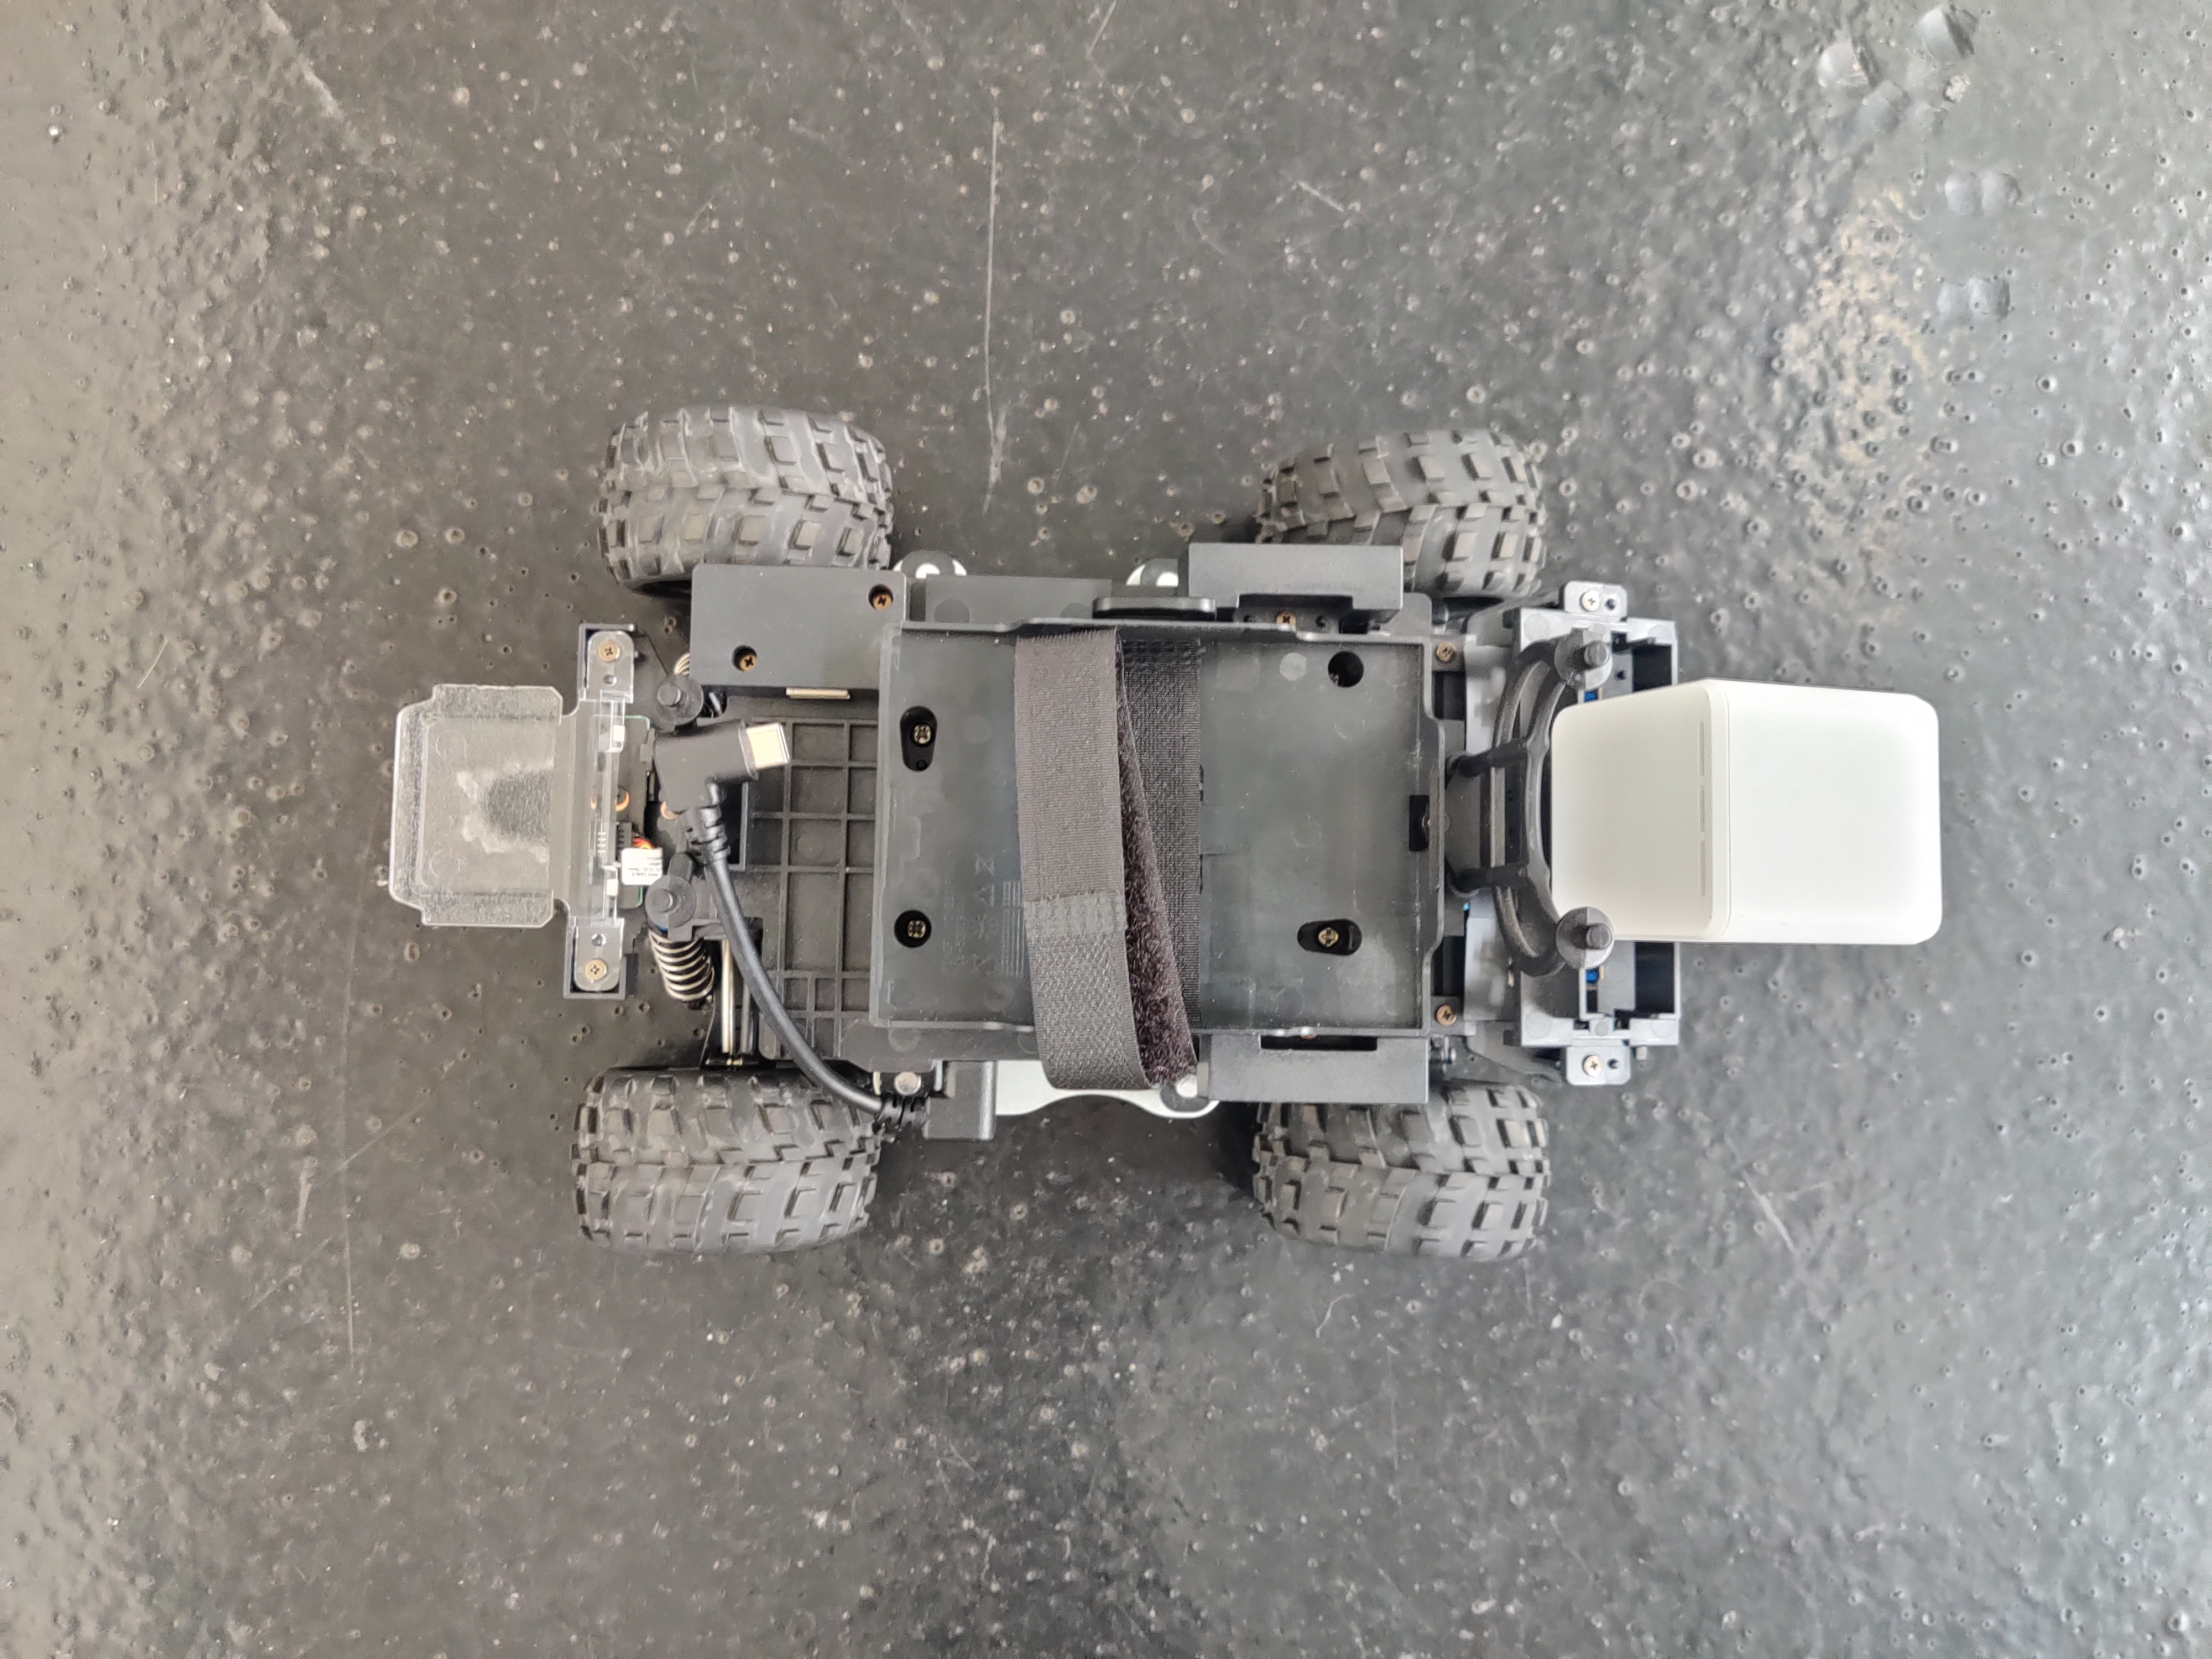
\includegraphics[width=.85\textwidth]{images/car_top_view.jpg}
    \caption{AWS DeepRacer Vehicle top view}
    \label{fig:vehicle_front}
\end{figure}

\subsection{Vehicle Steering}
The car an Ackermann front-wheel steering. The front wheels are mounted on suspensions which are connected with a second axis. This second axis, located behind the primary one is moved to the left or right and the wheels follow this movement. The steering pivots point inwards on the back of the front axle. They are connected via a bar called "track rod". By moving this bar to the left or right, the vehicles wheels are turned. The length of the track rod is slightly shorter than that of the axle. This leads to the wheels seemingly being misaligned, but this condition is intended.\repeatfootcite[p. 63]{Ackermann06}

\subsubsection{Advantage of Ackermann Steering}
The purpose of this steering mechanism is to minimize or in the best case completely eliminate wheel slip. The wheel alignment around a common turning point for both front wheels enables them to trace circles with different radii. Put differently, since the front wheels have different distances to the centre of the curve, in order to properly follow the intended path, they must turn at different angles.
% Include figure of Ackermann steering here

\subsubsection{Steering angle configuration}
The value which the agent uses as centre steering angle as well as the maximum steering angles can be configured via the web interface. This is necessary so that the car can drive in a straight line. Incorrectly configured steering can lead to severe hits in performance as the model has to compensate the drift caused by the misaligned wheels. In order to achieve the best results, the values defined in the action space before training should match the actions possible in real world scenarios. Alternatively, the steering configuration can be customised to fit the one defined in the action space. While fitting the simulation to the real world actions is likely to yield better results, it is often simpler to approximately configure the car's steering angle to match those defined in the action space.\repeatfootcite[p. 96]{AWS19}

\subsection{Vehicle and Compute-Module Batteries}
These batteries provide all parts with their necessary power. The battery supplying the compute-module is a common power bank with an USB-C connection. The one contained in the delivery provides 10 000 mAh of power. This is sufficient for operating it 3 to 4 hours. 

The second battery which powers steering and engine has less capacity and smaller in dimension. Its capacity is 7 500 mAh, which is enough for about 1 hours of continuous driving.

Replacements are confortable with ease, as both are easily accessible and replacement parts can be ordered online at reasonable prices. Especially the power bank used for the compute-module does not have to meet any other criteria than to fit on top of the vehicle and have sufficient capacity.

\section{Compute Module}
The upper component houses the ``brain'' of the car. The compute module consists of an Intel Atom
%todo: Fix trademark symbol
processor, 4 Gigabyte of RAM and 32 Gigabyte memory, which can be expanded via a SD card. This hardware is running Linux Ubuntu 16.04.3 with Intel OpenVINO\texttrademark{} and ROS\footnote{Robot Operating System} Kinetic. Apart from that the chassis offers 4 USB type A ports, 1 USB type C port, 1 Micro-USB port and one HDMI port. The USB type C port is used to supply the compute module with power, while the HDMI port offers the ability to connect a display and directly access the modules operating system.

As seen in figure \ref{fig:vehicle_front}, facing the left side of the car are three small LED lights. These lights are used to display the status of the power supply and the wireless LAN-connection. The first light indicates various states of the compute module, more precisely the states of the operating system running on the compute module. The following list shows the possible stages that this indicator can display.\repeatfootcite[p. 82 f.]{AWS19}
\begin{itemize}
    \item \textbf{Off} signals that the computer is turned off or is not supplied with sufficient power.
    \item \textbf{Blinking yellow} indicates the BIOS and the operating system being loaded after pressing the power button.
    \item \textbf{Steady yellow} means that the operating system is loaded and ready to use in a short amount of time.
    \item \textbf{Steady blue} shows that there is currently an application running on the compute module. This  light is also on while automated driving is activated.
    \item \textbf{Blinking blue} indicated that a software update is in progress.
    \item \textbf{Steady red} signals that an error occurred either during startup or while running an application.
\end{itemize}

\begin{figure}
    \centering
    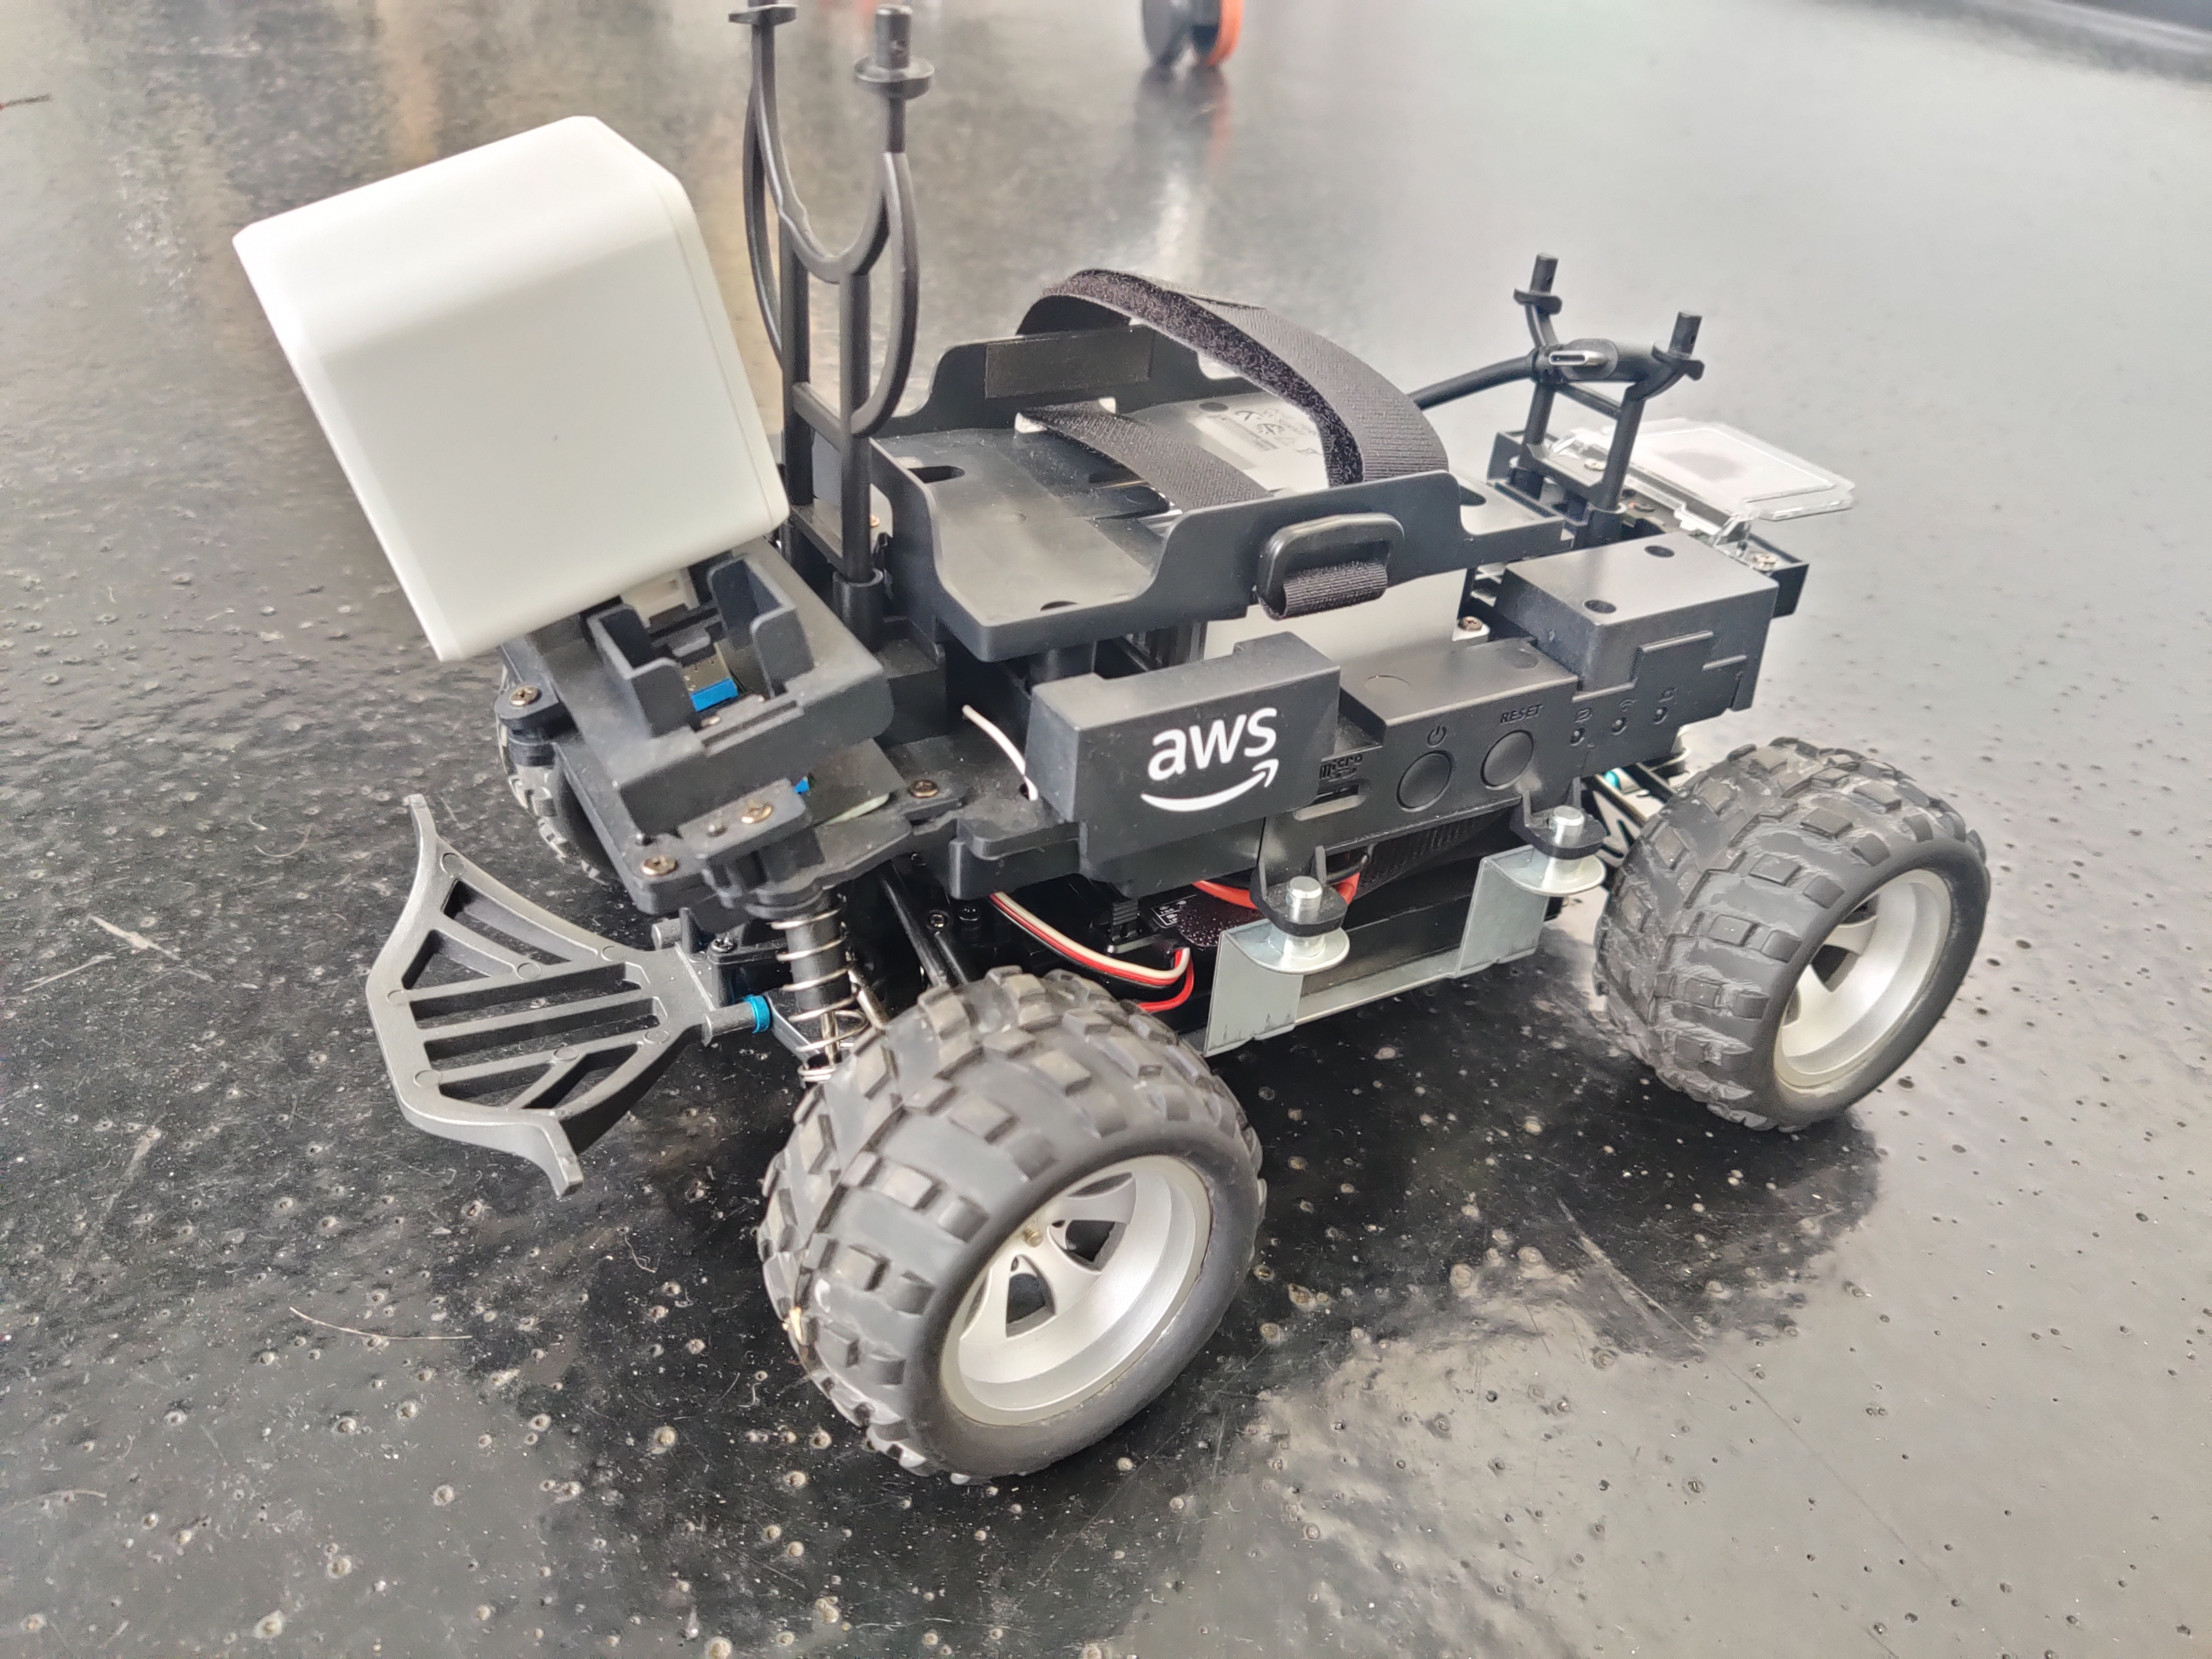
\includegraphics[width=.85\textwidth]{images/IMG_20201117_091128.jpg}
    \caption{AWS DeepRacer Vehicle side view}
    \label{fig:vehicle_side}
\end{figure}

\subsubsection{Web-Interface}
The compute module hosts its own web interface, from which the vehicle can be monitored, remotely controlled and configured. This interface is meant to be the main access point when working with the car. The website can be retrieved by accessing the IP-address of the car with a web browser. The address as well as the password which are required in order to access the configuration interface can be found on a label on the bottom of the car. The primary purpose of the website is configuration. This is indeed very useful as it removes the need to access the compute modules operating system directly. Without the web-interface, for every change it would be necessary to directly access the operating system by connecting a display, mouse and keyboard.

\begin{figure}
    \centering
    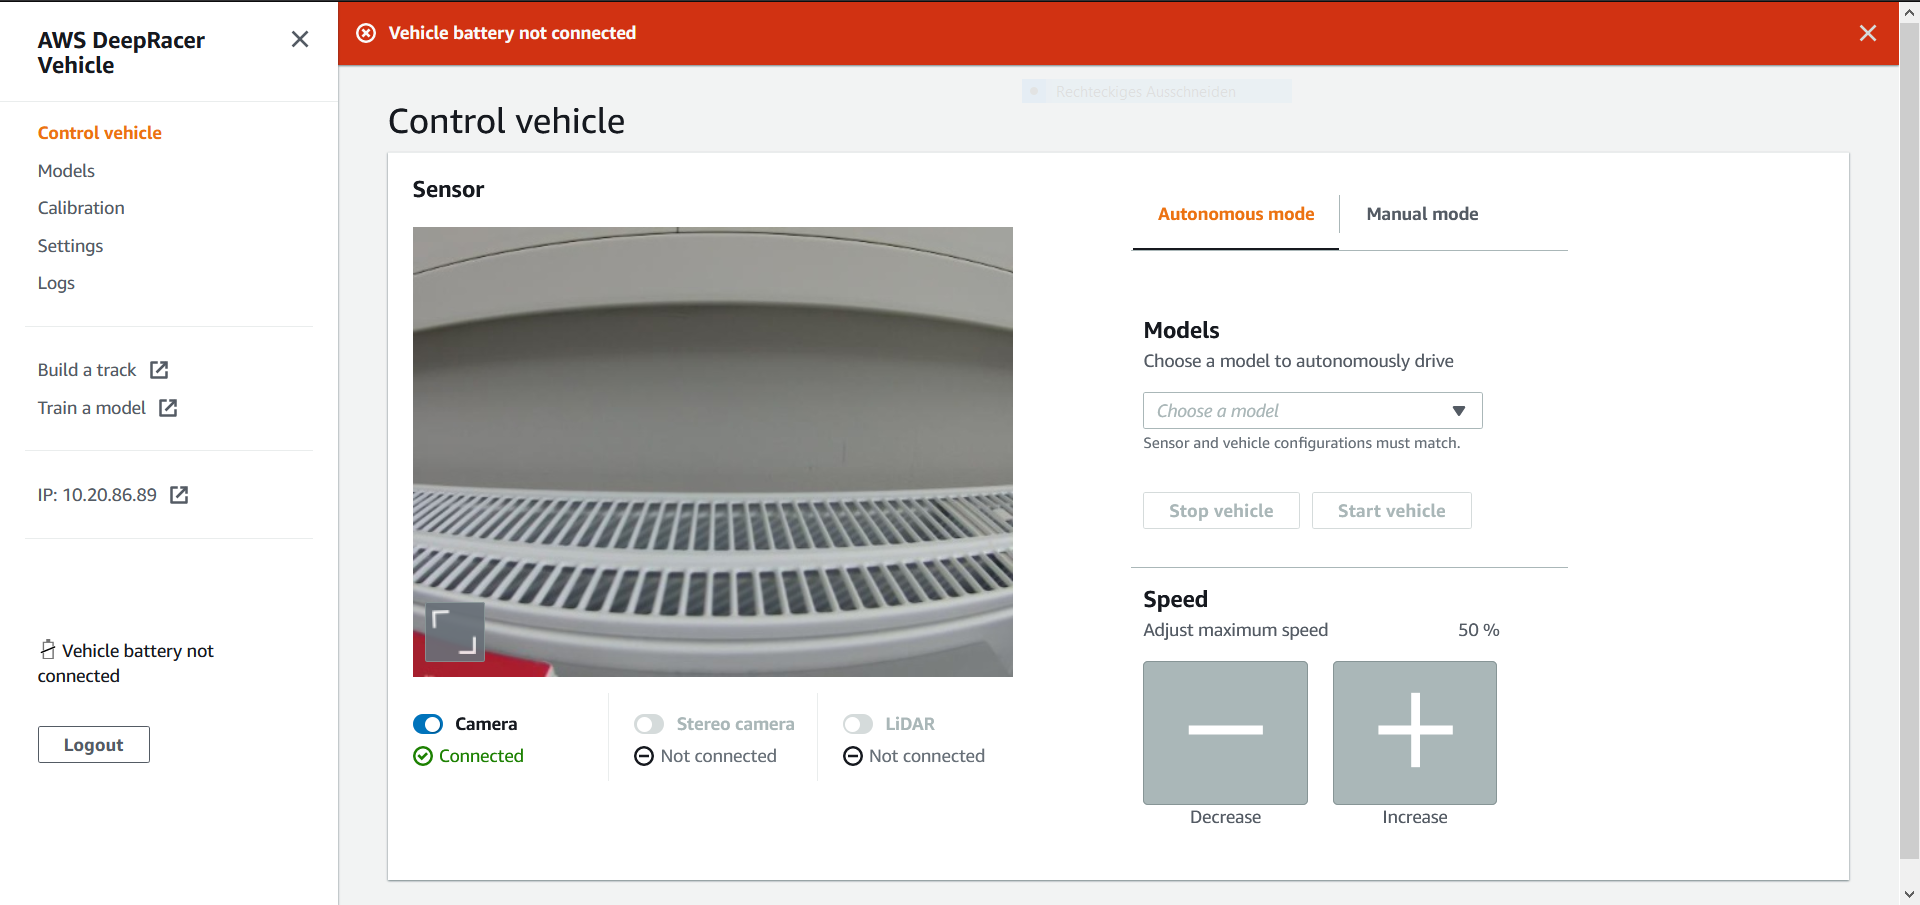
\includegraphics[width=.85\textwidth]{images/deepracer_console_1.png}
    \caption{DeepRacer Web interface}
    \label{fig:web_interface}
\end{figure}

\subsection{Configuration}
This section covers the configuration option possible via the web interface. There are two possible options that can be adjusted. The first one is the maximum and stopping speed. This setting determines how fast the car will drive when speed is set to maximum. The stopping speed sets the minimum power which the motor receives.

\subsection{Sensors}
In order to acquire the necessary information from the environment, the agent is outfitted with at least one sensor. Although we are only using the camera provided as a default sensor, this subsection covers other sensors available.

As mentioned, the default sensor provided is a single front-facing camera, connected via an USB-port at the front of the vehicle. The image provided by this part is the only information which the agent receives from its environment. This information is sufficient for the agent to traverse a marked track without obstacles or other vehicles. The only other information at our disposal is the sensor data from the electric motor and steering control. This provides us with information about the current speed and steering angle. Apart from that, all other information comes solely from the camera. Considering this, it is impressive that with a simple camera image, an entire vehicle can be controlled autonomously.

\section{Remote Control}
By default the DeepRacer vehicle offers the option for remote control via a virtual joystick on its web-interface. The direction as well as speed can be controlled this way. The input of this joystick is send to the car via an web-based application program interface (API). This API is hosted on the same web-server as the local interface seen in figure \ref{fig:web_interface}, this however shows the option for autonomous driving. Switching to manual control is done by selecting the manual mode tab located at the top right corner. After selecting the manual control tab, the website shows the joystick instead of the model selection menu. This can be seen in figure \ref{fig:manual_control}. Below the analogue-stick is the menu used for configuring the maximum speed. The current value is shown above the two buttons in percent. As an example, a value of 50 percent indicates that, when the analogue-stick is pressed all the way forward, the car drives at half of its highest possible velocity. This is the default way of remote controlling and sufficient enough for simple tests. If a more precise and ergonomic control mechanism is desired then it is necessary to directly access the underlying API. Accessing the  electric motor directly via ROS\footnote{Robot Operating System} is possible but not required. Driving this way has several disadvantages, most notably is it not possible to connect a game controller or similar device to the compute module, since the module does not have Bluetooth. Counteracting this can be achieved by using a computer as middle man. The game controller is connected to the computer, which sends the input to the vehicles manual control API.

\subsection{Web-API}
The application program interface is hosted on the same web-server as the rest of the local website. It is accessible behind the <IP-address>/api/ path. In order to access remote control, the correct credentials have to be put in and send to the /api/login endpoint. This then returns a session cookie which authorises the usage of other functionalities. The cookie has to sent with every request, otherwise it will return with an error stating an unauthorised access. The following list shows all endpoints relevant for remotely steering the car.

\begin{itemize}
    \item \textbf{Endpoint: start\_stop}: This API endpoint accepts the PUT method with a JSON-object with one field set. This field is named start\_stop and can take on either string of start or stop. It tells the car to either start or stop on the spot. This API call is required before beginning to drive.
    \item \textbf{Endpoint: manual\_drive}: Expects HTTP method PUT with a JSON-object containing the steering angle, speed and maximum speed.
\end{itemize}

The first API call is only used to start the car before driving. Without this, the vehicle will not move, even if told to do so by the second command. The endpoint manual\_drive is used to control the vehicle. It continuously receives requests which consist of three fields. The first field is named angle and defines the steering angle as a value ranging from -1 to 1. In this context, -1 is defined as a full left turn, while 1 represents a sharp right turn. The actual degree are set in the configuration menu under the maximum-steering-angle section. The second field is labeled throttle and represents the speed of the vehicle on percent. The percentage is taken from the maximum speed possible. A value of 0.5 is equal to half the maximum speed. The third field sets the maximum speed in metres per second. The actual speed can be calculated by multiplying the throttle field with the maximum speed.

\begin{figure}
    \centering
    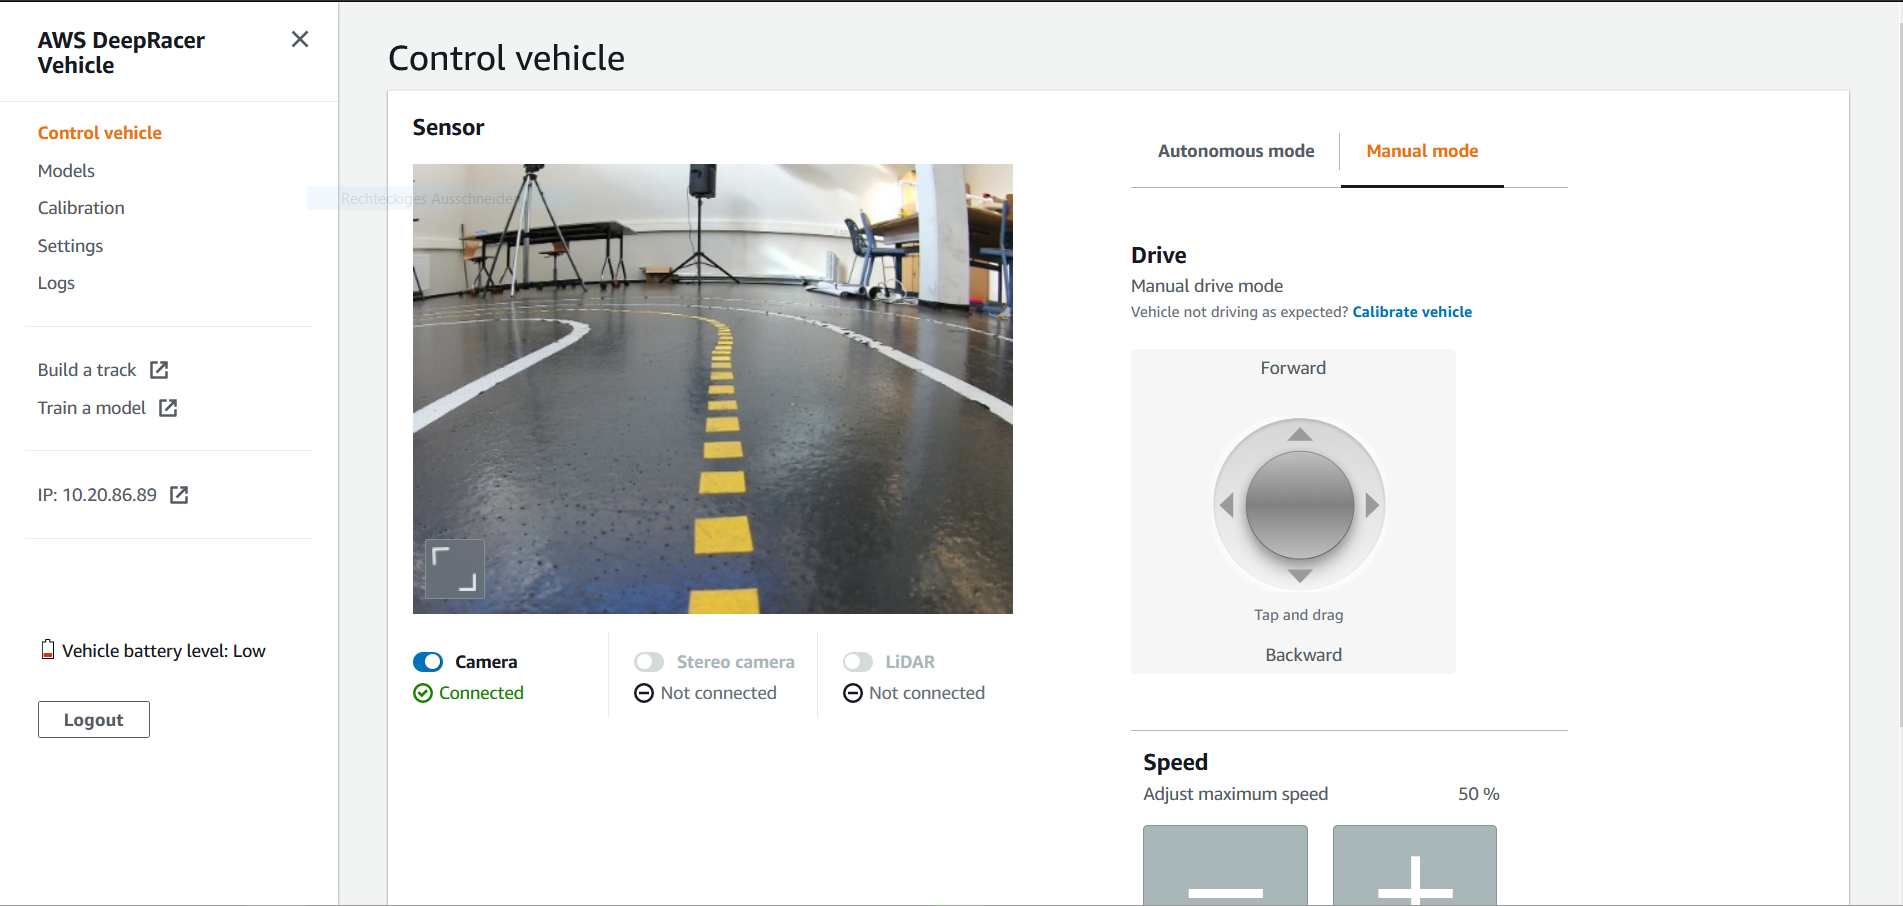
\includegraphics[width=.85\textwidth]{images/manual-control.png}
    \caption{Manual control interface}
    \label{fig:manual_control}
\end{figure}

\chapter{The physical Track}

Being able to drive along a simulation of the track is only a partial success. In order to prove successful, the trained algorithm is required to complete multiple runs on a real track using our DeepRacer vehicle. We decided on rebuilding the track used 2018 during the AWS re:Invent. The circular track starts with a 180° left turn, followed by a right-starting s-curve and continues on with two left turns back to the beginning. With a total width of 7.93 m and length of 5.18 m it impractical to paint it on a single, solid piece.

\begin{figure}
    \centering
    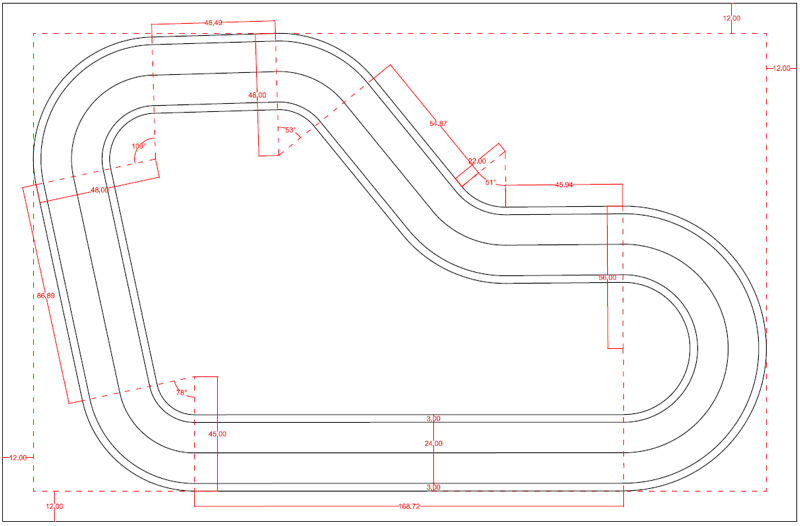
\includegraphics[width=.85\textwidth]{deepracer-track-2018-guideline.png}
    \caption{AWS re:Invent 2018 track}
    \label{fig:track}
\end{figure}

Before we considered building the track, we drew it on the floor in our robotics laboratory using duct tape. This was possible due to the floor being solid black, just like the road on the track. This variant has several drawbacks compared to a properly built track. Built like this the track is stationary and can not be removed without destroying parts of it. During removal it might even happen that the adhesive will leave stains on the floor, which then again need to be removed. The alternative, interlocking foam pieces, are transportable and more durable, as they can be easily removed and rebuild as needed. Their major drawback is the costs. While using duct tape as markings on the floor is cheaper and faster, using foam puzzles will be more efficient in the long run.

\section{The Material}
Choosing the right material for the track proved to be straightforward. It came down to either interlocking wooden composite plates or interlocking foam pieces. Foam pieces provide many advantages compared to other materials. They are lightweight and easy to transport. Durability and thickness are not as important, as the track is not meant to be stepped on and our car does not weight a lot. Far more important is the ability of the pieces to stick together. The tiles must not under any circumstances break away from each other, this could cause serious damage to the track and vehicle. Interlocking foam tiles are the cheapest material still meeting all criteria, with the only drawback being the cost.

\begin{table}
 \caption{Material price comparison}
 \label{tab:materials}
 \centering
 \setlength{\tabcolsep}{5mm}
 \def\arraystretch{1.25}
 \begin{tabular}{|r|r|c|c|}
 \hline
 \textbf{Material} & \textbf{Price} \\
 \hline\hline
 Black foam tiles & 299.85 € \\
 \hline
 Duct tape on floor & 59.85 € \\
 \hline
 \end{tabular}
 \end{table}

\subsection{Track and Field Colour}
The material is not the only factor we need to consider when building the track. Since our model is trained in a simulation with a specific colour scheme, we went to recreate this colour set in order to achieve the best performance. The road is the easiest to paint, as its colour is solid black with orange markings in the middle. The green area which covers most of the track is far more difficult to recreate. This leads to two options:
\begin{itemize}
    \item Black foam tiles, either paint the background green or leave it black
    \item Green foam tiles, where the road has to be drawn on
\end{itemize}

\chapter{LocalTraining}

\section{Local Training vs Cloud Training}
One of the major drawbacks of using the DeepRacer in a learning environment are the costs of training. Amazon offers easy, albeit functionally limited ways of training RL models in their cloud services. This sort of contradicts the intended use, as the DeepRacer is supposed to offer a simple and affordable entry into the ways of machine learning. Below is the pricing table. \footnote{Cited date 2020/08/20}
 \begin{table}
 \caption{Pricing for model training with AWS services.}
 \label{tab:services}
 \centering
 \setlength{\tabcolsep}{5mm}
 \def\arraystretch{1.25}
 \begin{tabular}{|r|r|c|c|}
 \hline
 \textbf{service} & \textbf{pricing} \\
 \hline\hline
 training and evaluation & 3.50 US\$ per hour \\
 \hline
 model storage & 0.023 US\$ per GB \\
 \hline
 \end{tabular}
 \end{table}
 In order to circumvent this cost barrier we -- like others before us -- began setting up a training environment on one of the more powerful computers in the robotics lab.
 The setup for local training is available on GitHub \footcite{https://github.com/aws-deepracer-community/deepracer}. In order to function properly the computer had to meet the following requirements:
 \begin{itemize}
 \item A Linux distribution, preferably Ubuntu
 \item NVIDIA grafic processor and proper drivers
 \item Docker
 \item Python
 \item Minio, a S3 simulator
 \end{itemize}
But after searching the internet we found a very cost efficient method, to train the model on our own computer. Given that in our robotics-lab we gain access to a "super-computer", which would train our models easily and fast we decided train our model by ourselves. Amazon doesnt provide a easy to use interface to download and upload models because they dont want to support you using your own servers and computers to train. Following this idea it seems that a lot of people worked their way around and made their own GUI's and interfaces. We tested two different GitHub projects, but were only left with one working so our decision fell on "deepracer for dummies" from alex schulz 

\section{Installing the Project Deepracer for dummies}
The author of this project relies heavily on another repository from the GitHub user crr0004 called Chris. Because his instructions were a little unclear and the project itself was lacing of feature and usability for the inexperienced end user such us, he decided to expand the project and make it easier to use. 
Before getting started with insalling the tools needed to run it on your machine you have to check if your computer meets the prerequisites:
At first you have to ensure that your operating system is Ubuntu 18.04 or higher, because some of the packages needed are only available on linux.
The next main point is that your system has to run on a Nvidia GPU and have CUDA/CUDNN installed and configured. If your machine doesnt provide a Nvidia GPU you are only able to train on your CPU which is much slower and takes a lot of time.
You also should have installed Docker aswell as the Nvidia-Docker runtime. This is needed for the training environment to gain access to the GPU and create new timelines.
Lastly vncviewer  has to be installed, because its the programm that controlos alle the interaction between the graphical user interface and the controllers from amazon.
If your system meets all the requiretments above you have to clone to run the init.sh script.
This could take up to 10 minites and all it does, it clone crr0004 reposetory, runs the needed scripts and creates and folderstructure including all the needed files, to manually adjust your code, train your model, and upload it to amazon.
After the setup process is finished i am going to get into a more detailed description on how the project handles the communication with the amazon cloud and how it handles the model.

 \section{Amazon Sagemaker}
 Sagemaker is a service amazon provides to create, train and handle machinelearning models. It handles the normally complicated  learning process to make it easier training multiple large models and dont have to worry about alle the tools and work processes that need to be done to learn efficent. Sagemaker contains a large toolset to handle all different components of machine learning. 
 %graphic
 SageMaker Studio is a webbased visual user interface that provides you full access, control and insight of alle the steps that need to be done to create train and analyze a model. You can upload own models and analyze results, make expiriecnes or provide it to get into production. 
SageMaker Ground on the other side, handles all the quick and easy to use data that is needed to train a model properly. Because a model is only as good as the data that is given to it, and with sagemaker ground you are able to manage all the trainig data.

\section{Amazon Robomaker}
Robomaker is a Cloud solution provided by amazon to create, simulate and test robotbased applications in large amounts. It gives you access to a fully scalable simulationinfrastructure for all you robots and your CI/CD-Integrations. Your are also given acces to an IDE to develop new Robotapplications and ROS extentions to make your robot coaloborate wit ROS.

\section{S3}
Amazon Simple Storage Service is a data Storage solution on whom you are able to store any kind of objects. It provides a high level of securaty, scalability and performence. You can use s3 for a large variaty of different usecases such as websites, mobile applications, IoT and Big Data Analytics.

\section{Errors occuring during the Installation process}
At our first try we installed all the needed tools and services, but made the mistake to forget to specify the nvidia cuda drivers. Altough the installation was succesfull, we were not able to train the model correctly, because the drivers didnt handle the communication between the invidual services well. The gui had a lot of bugs and was mostly unresponsive. We decided to uninstall all the drivers, files and services and get back to 0. We read the instarcutions one more time slowly and then relaised our human error. After repeating the whole installation process but including the wright driver version everything was working fine and we were able to start training our model. Furthermore we tried setting up the whole process on our laptops using ubunto in an virtial machine. But after discovering the cuda drivers wouldnt work out of a VM because they were not allowed to allocate memory on the physical graphics card, likewise because the hyperwiser wouldnt allow that, we tossed out that idea quickly
\chapter{Deepracer League}
Author: Sebastian Rohrer\newline
The AWS Deepracer League is a championship in which previously trained models can compete against each other. After each training session, there is the option to let the current model participate in an online race to see how it does against differently trained competitors. The Virtual Races are divided into Community Races and Online Leagues.\repeatfootcite{DeepracerLeague}

\section{Race-Types}
The Deep Racer supports three different Race-Types. Each Type has to be trained individually.

\subsection{Head-Head}
In the head-to-head qualifying, the racer completed a few laps while avoiding moving the AWS robot car on the track. At the end of this month, the top 32 qualifying rounds will enter the knockout rounds and fight side by side with other competitors.

\subsection{Object-Avoidance}
In the object avoidance competition, participants navigate the track while avoiding a specified number of fixed objects on the road. The fastest racer (including reset and collision time penalty) will be promoted to the chance to participate in the Champions League. This is the only Type that presupposes the Deep-Racer Evo because two cameras are needed to gain a stereo video feed to estimate lengths and depths.

\subsection{Time-Trial}
In the time trial, the racer must complete the required number of laps on the track. The racer with the fastest lap time (including heavy penalties for deviating from the track) will have a chance to compete for the Champions League.

\section{Online League}
All online races are directly accessible via the AWS cloud. Each Division is run by a different Race-Type and Map. After successfully participating in a division and getting upgraded to the next, the maps and Race-Types are getting more complicated.


\subsection{Open Division}
Any user can participate for free, who has trained his model for at least 5 minutes. This is the first and easiest tournament. The Race-Type is Time Trial, and the map is called Po-Chun Speedway. After finishing the race, the lap-time is compared to the other competitor's and the model is given a rank. Every month the top 10\% are promoted to the Pro Division. If needed, changes to the reward function can be made, and the model can participate as often as possible. 

\subsection{Pro Division}
In Pro Division, the Race-Type is Head-to-Head, but the other racers are swapped with bots. The map is called Po-Chun Super Speedway and is similar to the track on the open Division. 


\subsection{Pro Division Finals}
At the end of each month, the top 16 racers in the Pro department will compete with each other in the live racing console. This game will determine who will advance to the 2021 Champions League in the Pro Division Finals 2021 competition. The monthly Pro department winners will receive a free Pro Division Finals 2021 trip and participate in the Champions League, with a chance to win a machine learning education sponsorship worth US\$20,000. In both departments, digital rewards can be collected, including vehicle customisation and accessories, which will be released to participants every month after the winners are announced.
The Race-Type and Map are not yet announced, which forces the players to create multiple models and train their models on different tracks. This fact makes the finals as hard as possible for the players.  

\section{Community Races}
Instead of participating in an actual league, there is also the possibility to create an own race. With this option, it is possible to race against other players who do not participate in an online league. The Map and Race-Type are user-changeable. Today (11.03.2021), there are no available Community Races because the majority of the Racers is focused on real online tournaments.

\section{DeepRacer TV}
AWS DeepRacer TV is an Online Event in which famous Formula One Racer train their own DeepRacer and compete against Machine Learning Professionals. The event is hosted on the Amazon DeepRacer League Website and gets live-streamed on extensive Video-streaming services like YouTube and Twitch. The winner gets a ticket to the Pro Division Finals. The event is split into Weekly Rounds, and each competitor is filming their progress. 

\section{Participation conclusion}
As part of this thesis, we participated once in an open division to test how competitive the opponents are and how well the model needs to be trained to achieve good rankings.  

\subsection{Model}
For this experiment, a test model was created based on the hyperparameters shown on the table \ref{Sample Model Specifications}. The reward function has been reprogrammed using a waypoint algorithm that analyses existing waypoints on the map and calculates an ideal route.

\begin{listing}[H]
    \begin{minted}[frame=single, 
            framesep=3mm,
            linenos=true, 
            xleftmargin=21pt,
            tabsize=4]{Python}
    {
     
    waypoints = params['waypoints']
    closest_waypoints = params['closest_waypoints']
    heading = params['heading']

    reward = 1.0
    if progress == 100:
        reward += 100

    next_point = waypoints[closest_waypoints[1]]
    prev_point = waypoints[closest_waypoints[0]]
    
    track_direction = math.atan2(next_point[1] - prev_point[1], 
                                 next_point[0] - prev_point[0]) 
   
    track_direction = math.degrees(track_direction)
    direction_diff = abs(track_direction - heading)
    
    DIRECTION_THRESHOLD = 10.0
    malus=1

    if direction_diff > DIRECTION_THRESHOLD:
        malus=1-(direction_diff/50)
        if malus<0 or malus>1:
            malus = 0
        reward *= malus

    return reward
    \end{minted}
\end{listing}

The next and previous waypoint is fetched from an array containing all points of the whole route in the code example above. Then a line is calculated from the points, and based on this, their slope. This value is compared against a reference value, and based on that, the reward is paid out. The model was trained on the oval track for 1 hour and 48 minutes. The subsequent evaluation showed that in all 3 test trials, the car completed the track 100\% and all trials lasted between 23 and 24 seconds.

\subsection{Result}
Since this is an open division, it was not possible to train the model on the track in advance, as the point behind this is to program a solid algorithm that will perform well on all tracks. The DeepRacer finished 48th out of 50th competitors, with 6 minutes 17.831 seconds and 4 minutes 20.464 seconds off first place.  From the duration of the training and the algorithm, it can be said that in order to participate in the most superficial competition and achieve a good place, the respective model must be programmed very sophisticatedly and have many hours of training behind it. For beginners who want to gain experience with DeepRacer, it is best to participate in a community race or create one because the competition is high even in the most straightforward races.
\chapter{Schlussbemerkungen}
\label{cha:Schluss}

An dieser Stelle sollte eine Zusammenfassung der Diplomarbeit
stehen, in der auch auf den Entstehungsprozess, persönliche
Erfahrungen, Probleme bei der Durchführung,
Verbesserungsmöglichkeiten, mögliche %
Erweiterungen \usw\ eingegangen werden kann. War das Thema richtig
gewählt, was wurde konkret erreicht, welche Punkte blieben offen
und wie könnte man von hier aus weiter arbeiten?


\section{Lesen und lesen lassen}

Wenn die Arbeit fertig ist, sollten Sie diese zunächst selbst nochmals
vollständig und sorgfältig durchlesen, auch wenn man vielleicht das mühsam
entstandene Produkt längst nicht mehr sehen möchte. Zusätzlich ist sehr zu empfehlen, auch einer weiteren Person diese Arbeit anzutun -- man wird erstaunt sein, wieviele Fehler man selbst überlesen hat.



\section{Checkliste}

Abschließend noch eine kurze Liste der wichtigsten Punkte, an denen
erfahrungsgemäß die häufigsten Fehler auftreten (Tab.\ \ref{tab:checkliste}).


\begin{table}
\caption{Checkliste. Diese Punkte bilden auch die Grundlage der routine\-mäßigen
Formbegutachtung.}
\label{tab:checkliste}
\centering
\fbox{
\begin{minipage}{0.95\textwidth}
\medskip
\begin{itemize}
	\item[$\Box$] \textbf{Titelseite:} Länge des Titels (Zeilenumbrüche), Name,
	Abteilung, Datum.
	\item[$\Box$] \textbf{Erklärung:} vollständig Unterschrift.
	\item[$\Box$] \textbf{Inhaltsverzeichnis:} balanzierte Struktur, Tiefe, Länge
	der Überschriften.
	\item[$\Box$] \textbf{Kurzfassung/Abstract:} präzise Zusammenfassung, Länge,
	gleiche Inhalte.
	\item[$\Box$] \textbf{Überschriften:} Länge, Stil, Aussagekraft.
	\item[$\Box$] \textbf{Typographie:} sauberes Schriftbild, keine "`manuellen"'
	Abstände zwischen Absätzen oder Einrückungen, keine überlangen Zeilen,
	Hervorhebungen, Schriftgröße, Platzierung von Fußnoten.
	\item[$\Box$] \textbf{Punktuation:} Binde- und Gedankenstriche richtig gesetzt,
	Abstände nach Punkten (\va\ nach Abküzungen).
	\item[$\Box$] \textbf{Abbildungen:} Qualität der Grafiken und Bilder,
	Schriftgröße und -typ in Abbildungen, Platzierung von Abbildungen und Tabellen,
	Captions. Sind \emph{alle} Abbildungen (und Tabellen) im Text referenziert?
	\item[$\Box$] \textbf{Gleichungen/Formeln:} mathem.\ Elemente auch im Fließtext
	richtig gesetzt, explizite Gleichungen richtig verwendet, Verwendung von mathem.\ Symbolen.
	\item[$\Box$] \textbf{Quellenangaben:} Zitate richtig referenziert, Seiten- oder Kapitelangaben.
	\item[$\Box$] \textbf{Literaturverzeichnis:} mehrfach zitierte Quellen nur
	einmal angeführt, Art der Publikation muss in jedem Fall klar sein, konsistente
	Einträge, Online-Quellen (URLs) sauber angeführt.
	\item[$\Box$] \textbf{Sonstiges:} ungültige Querverweise (\textbf{??}), Anhang,
	Papiergröße der PDF-Datei (A4 = $8.27 \times 11.69$ Zoll), Druckgröße und
	-qualität.
\end{itemize}
\medskip
\end{minipage}%
}
\end{table}



\end{english}
%%%----------------------------------------------------------
%%%Anhang
\appendix
%\chapter{Technische Informationen}
\label{ch:TechnischeInfos}

\newcommand*{\checkbox}{{\fboxsep 1pt%
\framebox[1.30\height]{\vphantom{M}\checkmark}}}

\section{Aktuelle Dateiversionen}

\begin{center}
\begin{tabular}{|l|l|}
\hline
Datum & Datei \\
\hline\hline
\htldiplDate & \texttt{thldipl} \\
\hline
\htlDate       & \texttt{htl.sty} \\
\hline
\end{tabular}
\end{center}




\section{Details zur aktuellen Version}


Das ist eine völlig überarbeitete Version der Vorlage, die \texttt{pdf\-latex}
"`native"' und nicht (wie bisher) im DVI-Kompatibiliätsmodus verwendet. 
Der primäre Anlass für diesen Schritt war die Frage, wie man automatisch Metadaten im PDF-File ablegen kann, 
woraus sich allerdings eine Fülle von Änderungen ergeben haben, die in Summe die Arbeit mit LaTeX um 
Einiges leichter machen sollten. 

Es wird nunmehr als Ausgabe \emph{direkt} PDF erzeugt und (normalerweise) keine DVI-Datei mehr.
Der "`klassische"' DVI-PS-PDF-Modus ist allerdings weiterhin verfügbar (und auch notwendig, 
wenn man mit \texttt{psfrag} arbeiten möchte oder muss).

\subsubsection*{Verwendung unter Linux}
Was muss ich tun, um diese Version für meine Arbeit zu verwenden:
\begin{enumerate}
  \item Die Packete \textbf{texlive} und \textbf{texlive-lang-german} müssen
  installiert sein.
  \item \textbf{Eclipse} mit der Erweiterung \textbf{Texlipse} oder ein anderes
  \latex Frontend sollte installiert sein.
  \item Die Dateien \texttt{htldipl.cls} und \texttt{htl.sty} sind in das eigene
  Projektverzeichnis zu kopieren.
\end{enumerate}

\subsubsection*{Verwendung unter Windows}
Was muss ich tun, um diese Version für meine Arbeit zu verwenden:
\begin{enumerate}
\item \textbf{MikTeX 2.8} oder höher muss installiert sein.
%\item \textbf{SumatraPDF}%
%\footnote{\url{http://blog.kowalczyk.info/software/sumatrapdf/}} 
%Viewer muss installiert sein.
\item Die Dateien \texttt{htldipl.cls} und \texttt{htl.sty} sind in das eigene
Arbeitsverzeichnis zu kopieren.
%\item TeXniCenter-Profile für Sumatra importieren (aus beiliegender Datei \url{_tc_output_profiles_sumatra.tco}).
\end{enumerate}

\subsubsection*{Verwendung unter Mac~OS}

Unter Mac~OS wurde die aktuelle Vorlage noch nicht getestet. Der folgende Text bezieht sich auf die alte Vorlage und ist möglicherweise nicht mehr korrekt.

Diese Version sollte insbesondere unter \emph{MacTeX} problemlos laufen.
Was ist konkret zu tun, um die aktuelle Version unter Mac~OS zu verwenden:
\begin{enumerate}
\item \emph{MacTex} (2009 oder höher) muss installiert sein.
\item Ein PDF-Viewer muss verfügbar sein (\zB\ Mac~OS \emph{Preview}) -- \emph{TeXworks} hat eine eigenständige PDF Ausgabe inkludiert.
\item Die Zeichenkodierung des Editors muss auf ISO-8859-1 (Latin 1) gestellt sein.
\item Die Dateien \texttt{htldipl.cls} und \texttt{htl.sty} sind in das eigene
Arbeitsverzeichnis zu kopieren.
\end{enumerate}

\section{Einstellungen unter Windows} 
\label{sec:EinstellungAusgabeprofile}

Die folgenden Angaben beziehen sich auf eine bewährte Arbeitsumgebung unter MS Windows (XP, Vista, Win7) mit MikTeXund TeXnicCenter, mit folgenden Installationspfaden:
%
\begin{quote}
\verb!C:\Program Files\MiKTeX 2.8\! \\
%\verb!C:\Program Files\SumatraPDF\! \\
\verb!C:\Program Files\TeXnicCenter\! 
\end{quote}
%
Falls neuere Versionen dieser Komponenten installiert sind, müssen natürlich die nachfolgend angegebenen Pfade entsprechend modifiziert werden.


\subsection{TeXnicCenter-Ausgabeprofile}
\label{sec:TeXnicCenterUndMikTeX}

TeXnicCenter definiert den Verarbeitungsablauf des LaTeX-Dokuments anhand von Ausgabeprofilen, wobei die oben genannten Komponenten als externe Programme mit entsprechenden Argumenten aufgerufen werden.
Die Einstellung der Ausgabeprofile erfolgt in TeXnicCenter über das Menü
\textsf{Ausgabe}$\rightarrow$\textsf{Ausgabeprofile definieren...} (Abb.\ \ref{fig:techniccenter-profile-latex}). 
Die Profile werden (abhängig von der installierten Software) üblicherweise beim ersten Start von TeXnicCenter durch den zugehörigen "`Wizard"' voreingestellt. 


\begin{figure}
\centering\small
\setlength{\tabcolsep}{0pt}%
\begin{tabular}{c@{~}c}
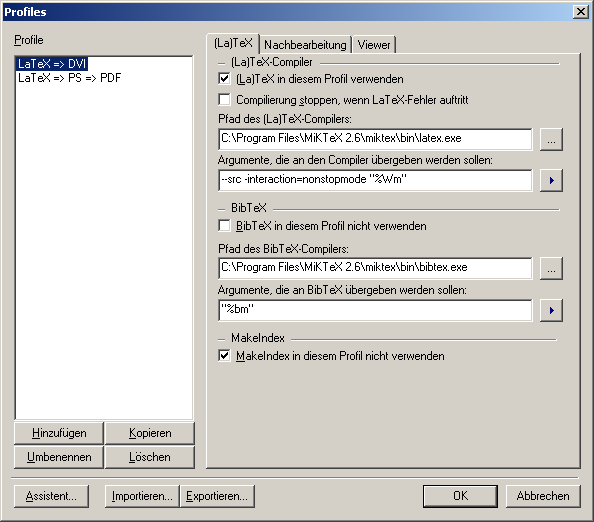
\includegraphics[width=0.49\textwidth]{techniccenter-profile-dvi-26} &
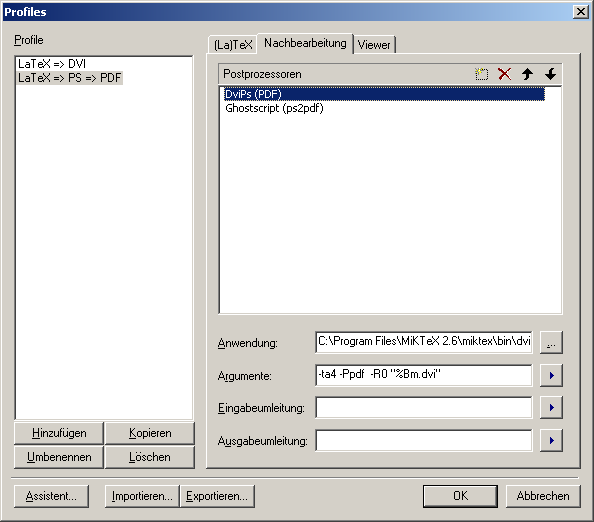
\includegraphics[width=0.49\textwidth]{techniccenter-profile-dvips-26} \\[4pt]
(a) & (b)
\end{tabular}
\caption{Spezifikation der Ausgabeprofile in TeXnicCenter.}
\label{fig:techniccenter-profile-latex}
\end{figure}

Für diese Vorlage wird die verwendung des Ausgabeprofiels \texttt{LaTeX => PDF} empfohlen.

%
%In der Datei \verb!tc_output_profiles_sumatra.tco! sind  folgende beiden "`maßgeschneiderten"' Ausgabeprofile für TexNicCenter angelegt (Import über \textsf{Build} $\rightarrow$ \textsf{Define Output Profiles ...}):
%\begin{itemize}
	%\item \verb!LaTeX => PDF (Sumatra)! -- Standard, direkte Erzeugung von PDF,
	%\item \verb!LaTeX => PS => PDF (Sumatra)! -- PDF "`klassisch"' via DVI und PS.
%\end{itemize}
%
%
%
%\subsubsection{Profil "`\texttt{LaTeX => PDF (Sumatra)}"'}
%
%Das ist das mit diesem Setup normalerweise verwendete Standardprofil.
%
%\paragraph{(La)Tex:}
%\begin{itemize}
  %\item Path to the (La)TeX compiler: \\
        %\begin{small} \verb!C:\Program Files\MiKTeX 2.8\miktex\bin\pdflatex.exe!\end{small}
  %\item Command line arguments to pass to the compiler:\\
%\begin{small}
   %\verb!-synctex=-1 -interaction=nonstopmode "%pm"!
%\end{small}
%\end{itemize}
%
%\paragraph{Postprocessor:} 
%leer, kein Postprocessor notwenig.
%
%\paragraph{Viewer:}
%\begin{itemize}
%\item Path of executable: \\
%\begin{small}
    %\verb!C:\Program Files\SumatraPDF\SumatraPDF.exe ! \\ 
    %\verb!-inverse-search "\"C:\Program Files\TeXnicCenter\TEXCNTR.EXE\" !\\
    %\verb!/ddecmd \"[goto('%f','%l')]\""!
%\end{small}
%%
%\item View project's output: \\
%\begin{small}
    %\checkbox\ Command line argument \\\
    %Command: \verb!"%bm.pdf"!
%\end{small}
%%
%\item Forward search:\\
%\begin{small}
    %\checkbox\ DDE command \\\
    %Command: \verb![ForwardSearch("%bm.pdf","%Wc",%l,0)]! \\
    %Server: \verb!SUMATRA! \\
    %Topic: \verb!Control!
%\end{small}
%\item Close document before running (La)TeX:\\
%\begin{small}
    %\checkbox\ Do not close
%\end{small}
%\end{itemize}
%
%
%
%
%\subsubsection{Profil "`\texttt{LaTeX => PS => PDF (Sumatra)}"'}
%
%Profil ausschließlich für den DVI-PS-Workflow (über DVI und PostScript).
%
%\paragraph{(La)Tex:}
%\begin{itemize}
  %\item Path to the (La)TeX compiler: \\
        %\begin{small} \verb!C:\Program Files\MiKTeX 2.8\miktex\bin\latex.exe!\end{small}
  %\item Command line arguments to pass to the compiler:\\
%\begin{small}
   %\verb!-synctex=-1 -interaction=nonstopmode "%pm"!
%\end{small}
%\end{itemize}
%
%\paragraph{Postprocessor:}
%\begin{itemize}
  %\item DviPS (PDF): \\
        %\begin{small} 
        %Executable: \verb!C:\Program Files\MiKTeX 2.8\miktex\bin\dvips.exe! \\
        %Arguments: \verb!-ta4 -P pdf -R0 "%Bm.dvi"!
        %\end{small}
  %\item Ghostscript (ps2pdf):\\
  		%\begin{small} 
        %Executable: \verb!C:\Program Files\gs\gs8.64\bin\gswin32c.exe! \\
        %Arguments: \verb!-q -dPDFSETTINGS=/prepress -sPAPERSIZE=a4 -dSAFER! \\
         %\verb!-dBATCH -dNOPAUSE -sDEVICE=pdfwrite -sOutputFile="%bm.pdf"! \\
         %\verb!-c save pop -f "%bm.ps"!
      %\end{small}
%\end{itemize}
%
%\paragraph{Viewer:}
%wie in Profil A. (\texttt{LaTeX => PDF (Sumatra)}).
	% Technische Ergänzungen
%\chapter{Inhalt der CD-ROM/DVD}
\label{app:cdrom}

\paragraph{Format:} 
		CD-ROM, Single Layer, ISO9660-Format%
\footnote{Verwenden Sie möglichst ein Standardformat, bei DVDs natürlich
eine entsprechende andere Spezifikation.}


\section{PDF-Dateien}
\begin{FileList}{/}
\fitem{_Diplomarbeit.pdf} Diplomarbeit mit Instruktionen (Gesamtdokument)
%
\end{FileList}


\section{\latex-Dateien}

\textbf{Achtung:} Die folgende Auflistung soll nur den Gebrauch dieser Vorlage
erleichtern. Es ist bei einer Diplomarbeit \ia\ \emph{nicht} notwendig, die zugehörigen \latex-Dateien aufzulisten (wohl aber projektbezogene Dateien, Ergebnisse, Bilder, Kopien von Online-Literatur etc.)!
%\paragraph{Pfad:} \url{/}
\begin{FileList}{/}
\fitem{_Diplomarbeit.tex} Diplomarbeit (Hauptdokument) %
\fitem{vorwort.tex} Vorwort %
\fitem{kurzfassung.tex} Kurzfassung %
\fitem{abstract.tex} Abstract %
\fitem{einleitung.tex} Kapitel 1 %
\fitem{diplomschrift.tex} Kapitel 2 %
\fitem{latex.tex} Kapitel 3
\fitem{abbildungen.tex} Kapitel 4 %
\fitem{formeln.tex} Kapitel 5 %
\fitem{literatur.tex} Kapitel 6 %
\fitem{drucken.tex} Kapitel 7 %
\fitem{word.tex} Kapitel 8 %
\fitem{schluss.tex} Kapitel 9 %
\fitem{anhang_a.tex} Anhang A (Source Code) %
\fitem{anhang_b.tex} Anhang B (Inhalt CD-ROM) %
\fitem{anhang_c.tex} Anhang C (Änderungen) %
\fitem{anhang_d.tex} Anhang D (Latex Quellcode) %
\fitem{messbox.tex} Messbox zur Druckkontrolle %
\fitem{literatur.bib} Literatur-Datenbank (BibTeX-File)
\end{FileList}

\begin{comment}
\section{Dokumentation}
%\paragraph{Pfad:} \url{/docs/}
\begin{FileList}{/docs/}
\fitem{caption2.pdf}  \texttt{caption} Paket %
\fitem{fancyhdr.pdf} "`Fancy Headers"' Paket %
\fitem{float.pdf}     \texttt{float}
Paket \fitem{gerdoc.pdf}    Kurzbeschreibung zu \texttt{german.sty}
und \texttt{ngerman.sty} \fitem{grfguide.pdf}  \texttt{graphicx} Paket
\fitem{l2kurz.pdf}    \latex-Anleitung (deutsch)
\fitem{lshort.pdf}    \latex-Anleitung (englisch)
\fitem{subfigure.pdf} \texttt{subfigure} Paket
\fitem{symbols-a4.pdf} Verzeichnis aller \latex-Symbole
\end{FileList}
\end{comment}

\section{Style/Class-Dateien}
%\paragraph{Pfad:} \url{/}
\begin{FileList}{/}
\fitem{htldipl.sty} Class-File für dieses Dokument
\fitem{htl.sty} Style-File für dieses Dokument
\fitem{algorithmicx.sty}  \texttt{algorithmicx} Paket (Version 1.1) 
\fitem{algpseudocode.sty} \texttt{algpseudocode} Paket 
\fitem{listings2.cfg} \texttt{listings2} Paket 
\fitem{listings2.sty} \texttt{listings2} Paket 
\fitem{lstaspects.sty} \texttt{listings2} Paket 
\fitem{lstdoc2.sty} \texttt{listings2} Paket 
\fitem{lstlanguages.sty} \texttt{listings2} Paket 
\end{FileList}


\section{Sonstiges}
\begin{FileList}{/images}
\fitem{*.ai} Original Adobe Illustrator-Dateien %
\fitem{*.fh11} Original Macromedia Freehand-Dateien %
\fitem{*.jpg} Original Rasterbilder %
\fitem{*.eps} Bilder und Grafiken im EPS-Format%
%\fitem{fonts-bakoma/} BaKoMa TrueType Fonts %
\end{FileList}
	% Inhalt der CD-ROM/DVD
%\chapter{Chronologische Liste der Änderungen}

\begin{sloppypar}
\begin{description}

\item[2018/07/02]
Überarbeitung für das Schuljahr 2018/19
\begin{itemize}
  \item Indixierung der Literatur nach Titel und Autor
  \item Allgemeiner Index für eigene Begriffe
  \item Software überarbeitet und auf den neuesten Stand gebracht
  \item Umstieg von biblatex auf biber
  \item Subfigure hinzugefügt
  \item Settings aus \_Diplomarbeit.tex ausgelagert
\end{itemize}


\item[2017/04/03]
FAQ hinzugefügt

\item[2017/03/28]
Anpassungen an sehr lange URLs in den Fußnoten

\item[2017/03/21]
Anpassungen an sehr lange Titel und Untertitel

\item[2016/10/20]
Neues Zitierformat (footcite)

\item[2016/04/04]
Umlaute in Codelistings möglich

\item[2015/10/11]
Dokumentationsseiten aus PDF Formular

\item[2015/10/07]
Umstieg von listings2 auf listingsutf8

\item[2015/10/06]
Syntax Highlighting umschaltbar zwischen Farbe und Schwarz / Weiß

\item[2015/09/29]
Neues Deckblatt

\item[2015/09/03]
Einseitig / Zweiseitig umschaltbar 

\item[2012/08/29]
Einstellbare Seitenränder durch das geometry Package

\item[2010/11/22]
Überarbeitung der originalen Vorlagen von Dr.\ Wilhelm Burger und Anpassung an
die Bedürfnisse einer HTL-
Wichtigste Änderungen:
\begin{itemize}
  \item Wechsel auf UTF8
  \item Wechsel auf listings2-beta
  \item Neue Code-Umgebungen für Python und C\#
  \item Vorlagen für Normen und Patente im Literaturverzeichnis
  \item Hinweise auf DVI-PS Workflow entfernt
  \item Kapitel zur automatischen \latex-Code erzeugung hinzugefügt
\end{itemize}
%
\end{description}

\end{sloppypar}

%\section*{To Do} 
%\begin{itemize}
%\item Literaturempfehlungen zum Schreiben von Diplomarbeiten
%\item Hinweise für Literatursuche (Bibliotheksverbund, CiteSeer,...)
%\end{itemize}



	% Chronologische Liste der Änderungen
%\chapter{\latex-Quellkode}
\label{app:latex}

\section*{Hauptdatei {\tt\_Diplomarbeit.tex}}

\begin{footnotesize}
\verbatiminput{_Diplomarbeit.tex}
\end{footnotesize}


%\vspace*{2cm}
\hrule
\hrule

\paragraph{Anmerkung:}
Das sollte nur ein \emph{Beispiel} für die Einbindung von Quellcode
in einem Anhang sein. Der \latex-Quellkode der eigenen
Diplomarbeit ist meist \emph{nicht} interessant genug, um ihn hier
wiederzugeben!

	% Quelltext dieses Dokuments

%%%----------------------------------------------------------
%Ausgabe der automatischen Zusatzdaten: Glossar, Index, Literaturverzeichnis
\clearpage
\printglossaries

\clearpage
\chapter*{Index}
\addcontentsline{toc}{chapter}{Index}
\printindex[allgemein]

\printindex

\printindex[name]

\printindex[title]


%Literaturverzeichnis
\clearpage
\addcontentsline{toc}{chapter}{\bibname}

\printbibliography


%%%----------------------------------------------------------

%%%Messbox zur Druckkontrolle
\chapter*{Messbox zur Druckkontrolle}



\begin{center}
{\Large --- Druckgröße kontrollieren! ---}

\bigskip

\Messbox{100}{50} % Angabe der Breite/Hoehe in mm

\bigskip

{\Large --- Diese Seite nach dem Druck entfernen! ---}

\end{center}



\end{document}
